\documentclass[%
master,         % тип документа
%natbib,         % использовать пакет natbib для "сжатия" цитирований
subf,           % использовать пакет subcaption для вложенной нумерации рисунков
href,           % использовать пакет hyperref для создания гиперссылок
colorlinks=false % цветные гиперссылки
%,fixint=false  % отключить прямые знаки интегралов
%,times         % шрифт Times как основной
]{disser}

\usepackage[
  a4paper, mag=1000,
  left=2.5cm, right=1.5cm, top=2cm, bottom=2cm, headsep=0.7cm, footskip=1cm
]{geometry}
\usepackage[T2A]{fontenc}
\usepackage[utf8]{inputenc}
\usepackage[english,russian]{babel}
%\usepackage{tabularx,longtable}
\ifpdf\usepackage{epstopdf}\fi

\usepackage{algorithm}
\usepackage{algpseudocode}
\renewcommand{\listalgorithmname}{Список алгоритмов}
\floatname{algorithm}{Алгоритм \textnumero\hspace{-3pt}}

% Номера страниц снизу и по центру
\pagestyle{footcenter}
\chapterpagestyle{footcenter}

% Точка с запятой в качестве разделителя между номерами цитирований
%\setcitestyle{semicolon}

% Использовать полужирное начертание для векторов
\let\avec\vec
\renewcommand{\vec}[1]{\boldsymbol{\mathbf{#1}}}

\addto\captionsrussian{\renewcommand\chaptername{}}
\addto\captionsrussian{\renewcommand\thechapterfont{\Large\bfseries}}
\addto\captionsrussian{\renewcommand\tocprethechapter{}}
\addto\captionsrussian{\renewcommand\prethechapter{}}
\addto\captionsrussian{\renewcommand\postthechapter{.}}

\renewcommand{\studentlabel}{Выполнила студентка гр. 971}

% Включать подсекции в оглавление
\setcounter{tocdepth}{1}

\graphicspath{{fig/}}

\begin{document}

% Переопределение стандартных заголовков
\def\contentsname{Содержание}
\def\conclusionname{Выводы}
\def\bibname{Список использованных источников}

\institution{Министерство образования и науки Российской Федерации
\\
Федеральное государственное автономное образовательное учреждение\\[-6pt] высшего профессионального образования\\[-6pt]
«Московский физико-технический институт\\[-6pt]
(государственный университет)»
\\
ФАКУЛЬТЕТ УПРАВЛЕНИЯ И ПРИКЛАДНОЙ МАТЕМАТИКИ\\[-6pt]
КАФЕДРА ВЫЧИСЛИТЕЛЬНОЙ МАТЕМАТИКИ
\\
(Специализация «Прикладные вычислительные модели\\[-6pt] и программные комплексы»)}

% Имя лица, допускающего к защите (зав. кафедрой)
\apname{{Холодов А.С}}

\title{Выпускная квалификационная работа\\[-6pt](магистерская диссертация)}

\topic{Маршевый метод решения задачи переноса излучения}

% Автор
\author       {Павлова Екатерина Сергеевна} % ФИО
\group        {971} % Группа
\coursenum    {03.04.01} % Номер направления
\course       {Прикладные математика и физика}
\masterprognum{\phantom{.}010991\phantom{.}} % Номер магистерской программы
\masterprog   {Прикладные вычислительные модели \\\hspace{16.7em} и программные комплексы}

% Научный руководитель
\sa      {Скалько Юрий Иванович}
\sastatus{к.ф.-м.н.}
% Второй научный руководитель
%\sasnd      {ФИО руководителя}
%\sasndstatus{д.~ф.-м.~н., ст.~н.~с.}

% Рецензент
\rev      {Колдоба Александр Васильевич}
\revstatus{д.~ф.-м.~н.}

% Город и год
\city{Москва}
\date{\number\year}

\maketitle

% Содержание
\tableofcontents
% Введение
\intro
Многие современные задачи численного моделирования высокотемпературных процессов сталкиваются с необходимостью учета процессов излучения. Среди них задачи, связанные с моделированием звездных атмосфер и межзвездного вещества, динамикой высокотемпературной плазмы, проектированием теплозащиты спускаемых аппаратов. Современные постановки этих задач существенно сложны и опираются, как правило, на трехмерное пространственное описание процессов. В то же время, в этих задачах излучение может иметь значительную и, даже, определяющую роль.

Сама по себе задача нахождения поля излучения является довольно сложной. В общем случае, интенсивность излучения является функцией координат, времени, направления и частоты излучения. Решение полной задачи — крайне сложная задача. Но влияние излучения на другие процессы обычно описывается некоторыми интегральными характеристиками интенсивности излучения. Поэтому, на практике, вместо полной постановки используется некоторым способом осредненная (по частотам, направлениям)
приближенная постановка, имеющая существенно меньшую размерность.

Развитие численных методов для решения уравнения переноса излучения проходило с 50-х годов прошлого столетия. В то время разрабатывались методы, учитывающие ту или иную симметрию задачи, сводящую ее к эффективно одномерной или двумерной. Однако, эти методы совершенно непригодны для современных задач, и не являются универсальными.
% Глава 1
\chapter{Постановка задачи}
Целью  данной работы является создание маршевого (безытерационного) вычислительного алгоритма для решения задачи переноса излучения на неструктурированных трехмерных сетках. 

Основными задачами, решаемыми в данной работе, являются:
\begin{itemize}
\item Разработка алгоритма упорядочения - основа маршевого метода
\item Разработка метода повышенного порядка аппроксимации
\item Сравнение результатов, полученных различными методами.
\end{itemize}

В работе \cite{skalko_2014} приведен алгоритм упорядочения, но он предазначен исключительно для триангуляций, удовлетворяющих условию Делоне. При разработке метода повышенного порядка аппроксимации неизбежно возникает проблема обеспечения <<физичности>> решения, которую можно обеспечить при монотонности используемой схемы.
\section{Математическая модель}
Поле излучения, заполняющего пространство, описывается распределением интенсивности излучения по частотам, в пространстве и по направлениям переноса лучистой энергии. Пусть $f(\nu, \vec r, \vec \Omega, t)d\nu d\vec r d \vec \Omega \, $ есть число световых квантов в спектральном интервале от $ \nu$ до $ \nu + d\nu$, находящихся в момент $t$ в элементе объема $d\vec r$ около точки $\vec r$ и имеющих направление движения в элементе телесного угла $d\vec \Omega$ около единичного вектора $\vec \Omega$. 
Каждый квант обладает энергией $h \nu$ и движется со скоростью $c$, поэтому величина 
\begin {equation}
I_{\nu} (\vec r, \vec \Omega, t)d \nu d\vec \Omega = h\nu c f (\nu, \vec r, \vec \Omega, t)d\nu d\vec{\Omega}
\end {equation}
есть количество лучистой энергии в спектральном интервале $d\nu$, протекающей в $1 \text{ сек}$ через площадку в $1 \text{ см}^2$, помещенную в точке $\vec r$ перпендикулярно к направлениям распространения энергии, которые лежат в элементе телесного угла $d\vec\Omega$ около вектора $\vec \Omega$. Задание функций $I_{\nu}$ или $f$ полностью определяет поле излучения. Количество лучистой энергии, заключенной  спектральном интервале $d\nu$ и находящейся в $1 \text{ см}^3$ пространства в точке $\vec r$ в момент $t$, или спектральная плотность излучения, равно:
\begin {equation}
U_\nu (\vec r, t) = h \nu \int_{4 \pi} f d \Omega = \frac{1}{c} \int_{4\pi} I_{\nu} d\Omega.
\end {equation}

Вектор спектрального потока равен 
\begin {equation}
\vec S_{\nu} = \int_{4\pi} I_{\nu}\vec\Omega d\Omega,
\end {equation}
где $\vec\Omega$ - единичный вектор направления движения квантов. 
Полные интенсивность, плотность и поток излучения получаются из спектральных интегрированием их по всему спектру частот:
\begin {equation}
I = \int_0^\infty I_{\nu} d\nu, \quad U = \int_0^\infty U_{\nu}d\nu, \quad \vec S =  \int_0^\infty \vec S_{\nu}d\nu.
\end {equation}
\section{Уравнение переноса}
Рассмотрим баланс излучения в элементарном цилиндре \ref{fig:1} с площадью основания $d\sigma$ и высотой $ds$, расположенном в данной точке пространства таким образом, что направление $\vec\Omega$ совпадает с образующей цилиндра и перпендикулярно к его основаниям. За время $dt$ в левое основание втекает количество излучения $I_{\nu} (\vec\Omega, \vec r,t)d\sigma dt$. Из правого основания за тот же промежуток времени вытекает количество излучения $(I_{\nu} + dI_{\nu})d \sigma dt$.

\begin{figure}[ht!]
\centering{
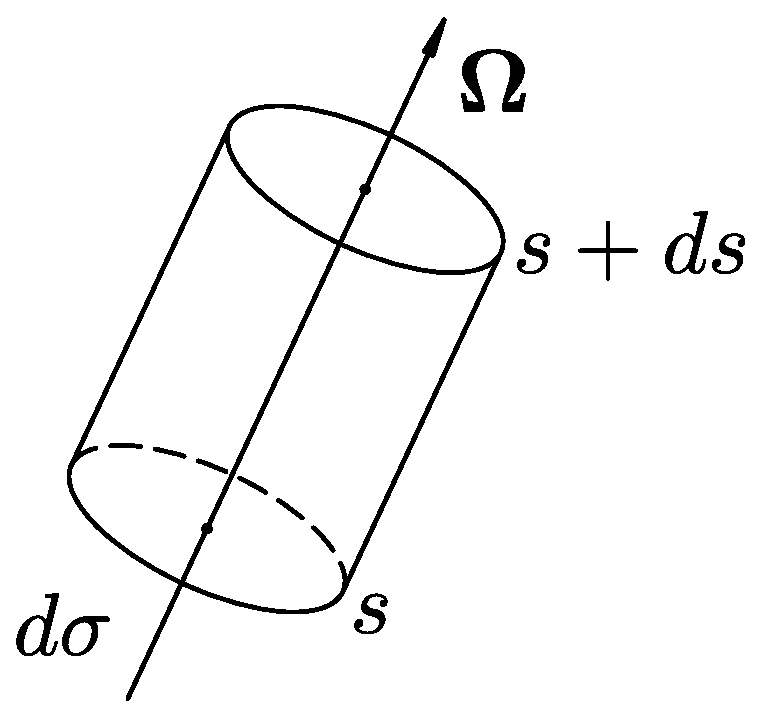
\includegraphics[width = 0.3\textwidth]{cylinder.eps}
}
\caption{К выводу уравнения переноса излучения}
\label{fig:1}
\end{figure}

Интенсивность $I_{\nu}$ есть функция координат и времени. Приращение интенсивности пучка света при переходе от левого основания к правому складывается из локального приращения за время прохождения светом пути $ds$ и из приращения при переходе от координаты $s$ к координате $s+ds$ в данный момент времени, 
\begin {equation}
dI_{\nu}  = \frac{\partial I_{\nu}}{\partial t } \frac{ds}{c}+\frac{\partial I_{\nu}}{\partial s}ds.
\end {equation}

Введем коэффициент поглощения $\varkappa_\nu$ таким образом, что количество лучистой энергии в интервале частот $d\nu$ и интервале направлений $d\vec\Omega$, поглощаемой в $1 \text{ см}^3$ в  $1 \text{ сек}$, равно
\begin {equation}
I_{\nu}d\nu d\vec\Omega \varkappa_{\nu}.
\label {3}
\end {equation}
Обозначим плотность самопроизвольного испускания $j_\nu$. То есть количество энергии, самопроизвольно испускаемой веществом  в $1 \text{ см}^3$ в  $1 \text{ сек}$ интервале $d\nu d\vec\Omega$, равно $j_{\nu}d\nu d\vec\Omega$. Помимо самопроизвольного испускания также существует так называемое вынужденное испускание. Вероятность вынужденного испускания кванта данной частоты и данного направления пропорциональна имеющейся в данной точке пространства интенсивности излучения той же частоты и того же направления. Известно \cite{zeld_2013}, что полная вероятность испускания данных квантов пропорциональна величине $1+n$, где $n = c^2I_{\nu}/2h\nu^3$. Таким образом, полное количество излучения, испускаемого в $1 \text{ сек}$ в $1 \text{ см}^3$ в интервале $d\nu d\vec\Omega$, равно 
\begin {equation}
j_{\nu} d\nu d\vec\Omega \left(1+\frac{c^2}{2h\nu^3}I_{\nu}\right).
\label{4}
\end {equation}
Первое слагаемое в скобках соответствует спонтанному испусканию, а второе - вынужденному. 

Количество излучения, испущенного в цилиндре за время $dt$, согласно формуле \eqref{4}, равно
\begin {equation}
j_{\nu}\left(1 + \frac {c^2}{2h\nu^3}I_{\nu}\right)d\sigma ds dt.
\end {equation}
Поглощается в нем за то же время количество излучения $\varkappa_{\nu} I_{\nu}d\sigma dsdt$. Составляя баланс и поделив полученное выражение на произведение дифференциалов $d\sigma dsdt$, получим уравнение
\begin {equation}
\frac{1}{c} \left(\frac{\partial I_{\nu}}{\partial t} + c \vec \Omega \nabla I_{\nu}\right) = j_{\nu} \left(1 + \frac {c^2}{2h\nu^3}I_{\nu}\right) - \varkappa_{\nu}I_{\nu}.
\label{1}
\end {equation}

Преобразуем правую часть уравнения \eqref{1}, объединив вместе члены, отвечающие поглощению и вынужденному испусканию, поскольку они оба пропорциональны неизвестной функции координат и времени - интенсивности излучения. 

Рассмотрим среду, находящуюся в состоянии термодинамического равновесия при постоянной температуре $T$. В стационарных условиях поле излучения также равновесно. Спектральная функция плотности равновесного излучения $U_{\nu p}$ подчиняется закону Планка. Количество энергии равновесного излучения частоты $\nu$ в $1 \text{ см}^3$, приходящееся на единичный интервал частот, равно
\begin {equation}
U_{\nu p} = \frac{8 \pi h \nu^3}{c^3} \frac {1}{e^{\frac{h\nu}{kT}} - 1}
\end {equation}
В силу изотропии спектральная интенсивность равновесного излучения равна
\begin {equation}
I_{\nu p} = \frac{cU_{\nu p}}{4\pi} = \frac{2h\nu^3}{c^2}\frac{1}{e^{\frac{h\nu}{kT}} - 1}
\label{5}
\end {equation}

В состоянии термодинамического равновесия испускание и поглощение квантов данных частоты и направления в точности компенсируют друг друга, так что выражения \eqref{3} и \eqref{4} следует приравнять, причем интенсивность излучения $I_{\nu}$ заменить при этом равновесной величиной $I_{\nu p}$. 
Принимая во внимание формулу \eqref{5} для равновесной интенсивности, найдем, что отношение лучеиспускательной способности любого вещества к его коэффициенту поглощения есть универсальная функция частоты и температуры:
\begin {equation}
\frac{j_{\nu}}{\varkappa_{\nu}} =  \frac{I_{\nu p}}{1+\frac{c^2}{2h\nu^3}I_{\nu p}} = \frac{2h\nu^3}{c^2}e^{-\frac{h\nu}{kT}}.
\label{6}
\end {equation}

Это отношение представляет собой одну из форм закона Кирхгофа. Формулу \eqref{6} удобно переписать в виде
\begin {equation}
j_{\nu} = I_{\nu p}\varkappa_{\nu}\left(1-e^{-\frac{h\nu}{kT}}\right).
\label{7}
\end {equation}

В новой трактовке закон Кирхгофа \eqref{7} приобретает форму
\begin {equation}
j_{\nu} = \varkappa'_{\nu}I_{\nu p}, \quad \varkappa'_{\nu} = \varkappa_{\nu}\left(1 - e^{-\frac{h\nu}{kT}}\right).
\end {equation}

Введем при этом в множитель перед $I_{\nu}$ в члене вынужденного испускания вместо коэффициента излучения $j_{\nu}$ его выражение через коэффициент поглощения, в которое подставим формулу \eqref{5} для равновесной интенсивности. Правая часть уравнения \eqref{1} примет вид 
\begin {equation}
j_{\nu} - \varkappa_{\nu}\left(1 - e^{-\frac{h\nu}{kT}}\right)I_{\nu}.
\end {equation}
Отсюда видно, что вынужденное испускание можно трактовать как некое уменьшение поглощения: часть квантов поглощается и тут же испускается снова с той же частотой и в том же направлении, причем вероятность этого <<переизлучения>> равна $e^{-\frac{h\nu}{kT}}$. Можно считать, что коэффициент поглощения имеет несколько меньшую величину:
\begin {equation}
\varkappa'_{\nu} = \varkappa_{\nu}\left(1 - e^{-\frac{h\nu}{kT}}\right).
\end {equation}

Взаимодействие излучения с веществом можно представлять так, как будто существует только спонтанное испускание и эффективное поглощение, описываемое коэффициентом $\varkappa'_{\nu}$, исправленным на вынужденное испускание. 

Вводя это выражение в правую часть уравнения переноса \eqref{1} запишем уравнение в следующей форме:
\begin {equation}
\frac{1}{c}\frac{\partial I_{\nu}}{\partial t} + (\vec\Omega \nabla) I_{\nu} = \varkappa'_{\nu} (I_{\nu p} - I_{\nu}).
\label{2}
\end {equation}

Будем в дальнейшем понимать под $\varkappa_\nu$ коэффициент поглощения $\varkappa_\nu'$, т.е. подправленный на спонтанное излучение.
\section {Граничные условия}
Дополним уравнение \eqref{2} граничными условиями \cite{chetv_1985}. Они должны определять только излучение, приходящее извне в исследуемый объем. Мы ограничиваемся случаем заданного излучения извне, поскольку условия отражения связывают уравнения переноса в разных направлениях. В случае выпуклых областей для направлений $\vec\Omega$, выходящих в рассматриваемую область, имеет место неравенство $(\vec\Omega, \vec n) < 0$, где $\vec n$ -- вектор внешней нормали к границе $G$ (см рис \ref{fig:6}).
\begin{figure}[ht!]
	\centering{
		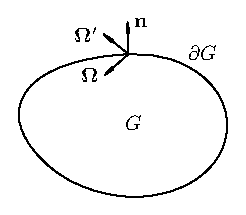
\includegraphics[width = 0.4\textwidth]{bord.eps}
	}
	\caption{Граничные условия для выпуклых областей. На участке границы $\partial G$ происходит зеркальное отражение фотонов}
	\label{fig:6}
\end{figure}

Граничное условие на границе $G$ примет вид
\begin {equation}
I_\nu (G, \vec\Omega, \nu, t) = I_\nu^*(G, \vec\Omega, \nu, t), \quad (\vec\Omega, \vec n) < 0.
\end {equation}
Здесь $I_\nu^*$ - известная функция, определяющая приходящее извне излучение. В работе используется граничное условие вида
\begin {equation}
I_\nu (G, \vec\Omega, \nu, t) = 0, \quad (\vec\Omega, \vec n) < 0.
\end {equation}
Это условие соответствует тому, что источники излучения находятся только внутри рассматриваемой области.

Иногда часть границы области $\partial G$ отражает выходящее из объема излучение. Простейшим случаем отражения является зеркальное отражение. При этом отражение происходит по законам классической оптики:
\begin {equation}
I_\nu (G, \vec\Omega, \nu, t) = \delta I_\nu(\partial G, \vec\Omega_1, \nu, t), 
\end {equation}
где $\vec\Omega_1 = \vec\Omega - 2\vec n( \vec\Omega\vec n)$ --- симметричное к $\vec\Omega$ относительно нормали $\vec n$ направление, $\delta$ --- коэффициент отражения, $0 \leqslant \delta \leqslant 1$.
\section{Аналитическое решение уравнения переноса}
Найдем формальное решение уравнения переноса излучения, рассматривая величины, зависящие только от состояния вещества $I_{\nu p}(T)$, $\varkappa_{\nu}(T, \rho)$, как известные функции координат и времени. Рассмотрим сначала для простоты стационарный случай, когда распределения температуры и плотности, а также поле излучения не зависят от времени. Будем интересоваться излучением в точке $\vec r$ тела с направлением распространения $\vec \Omega$ (см. рис. \ref{fig:2}). 
\begin{figure}[ht!]
\centering{
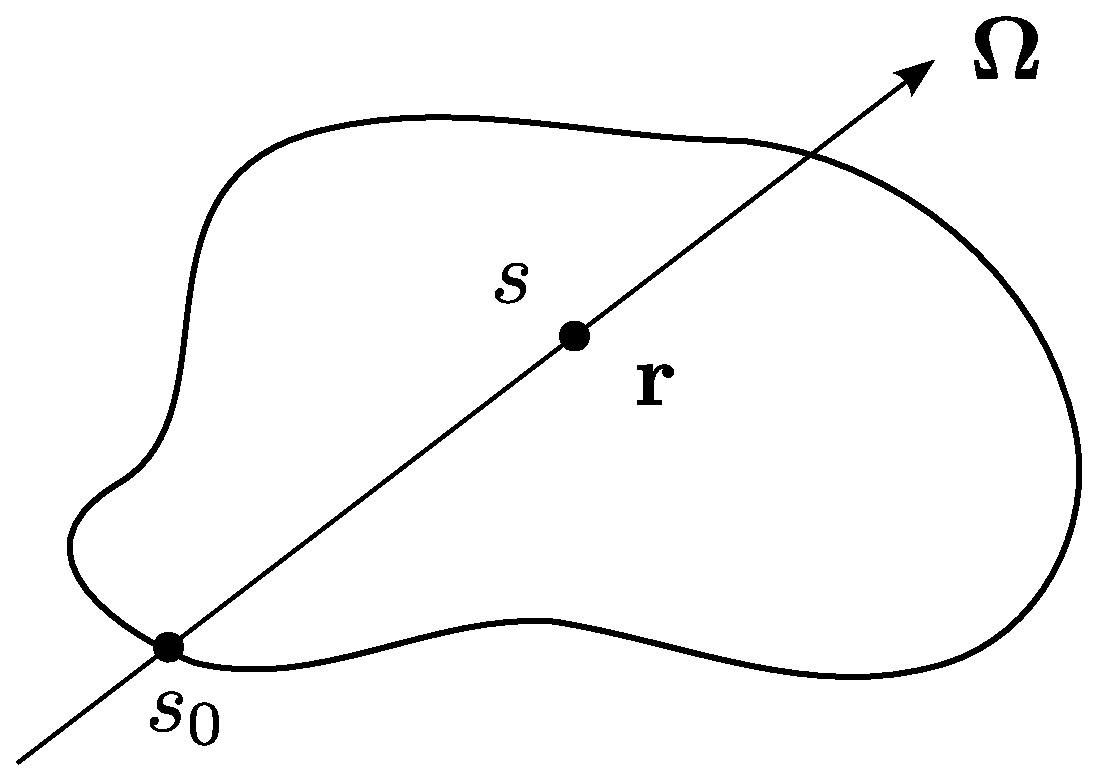
\includegraphics[width = 0.4\textwidth]{analytic.eps}
}
\caption{Схема, поясняющая пределы интегрирования в формуле для точного решения}
\label{fig:2}
\end{figure}
Проведем луч через данную точку в данном направлении и обозначим координату вдоль луча через $s$. Замечая, что дифференциальное выражение в левой части уравнения переноса \eqref{2} представляет собой полную производную от интенсивности вдоль луча распространения, перепишем уравнение в виде
\begin {equation}
\frac{dI_{\nu}}{ds} + \varkappa_{\nu}I_{\nu} = \varkappa_{\nu}I_{\nu p}.
\end {equation}
Это уравнение можно рассматривать как обыкновенное линейное уравнение относительно интенсивности вдоль луча. Решение его есть:
\begin {equation}
I_{\nu}(s) = \int_{s_0}^s\varkappa_{\nu}I_{\nu p} \exp\Big[-\int_{s'}^s\varkappa_{\nu}ds''\Big]ds' + I_{\nu,0} \exp\Big[-\int_{s_0}^s \varkappa_{\nu}ds''\Big].
\label{8}
\end {equation}

Здесь $I_{\nu}(s)$ - интенсивность $I_{\nu}(\vec r, \vec\Omega)$, которая рассматривается как функция координаты $s$ вдоль луча. Интегрирование по лучу ведется от границы тела $s_0$ (как показано на \ref{fig:2}). Через $I_{\nu, 0}$ обозначена константа интегрирования, которая имеет смысл значения интенсивности излучения на границе в точке $s_0$.

Величина
\begin{equation}
\tau(s_1, s_2) = \int_{s_1}^{s_2} \varkappa_\nu ds
\end{equation}
называется оптической толщиной вдоль луча от точки $s_1$ до точки $s_2$. Будем называть область от $s_1$ до $s_2$ оптически плотной, если $\tau(s_1, s_2) \gg 1$ и оптически прозрачной, если $\tau(s_1, s_2) \ll 1$.
С использованием оптической толщины формула \eqref{8} для интенсивности в точке $s$ может быть записана в виде
\begin{equation}
I_\nu(s) = \int_{s_0}^s \varkappa_\nu I_{\nu p} e^{-\tau(s', s)} ds'
+ I_{\nu,0} e^{-\tau(s_0, s)}
.
\label{eq:8_5}
\end{equation}
% Глава 2
\chapter{Численный метод}

\section{Общие положения метода коротких характеристик}
Уравнение \eqref{2} при каждом $\nu$ имеет гиперболический тип и семейство характеристик, которые просто являются характеристиками одномерных уравнений переноса вдоль направления $\vec\Omega$ 
\begin {equation}
\vec r - \vec r_0 = \vec \Omega c(t-t_0).
\end {equation}

Рассмотрим нестационарное уравнение переноса
\begin {equation}
\frac{1}{c}\frac{\partial I_{\nu}}{\partial t} + (\vec\Omega \nabla) I_{\nu} + \varkappa_\nu I_\nu = \varkappa_{\nu} I_{\nu p}.
\end {equation}

Выберем некоторым образом на единичной сфере набор направлений $\Theta = \{\vec\omega_i\}_1^n$. Для каждого направления уравнение является одномерным уравнением переноса, причем между собой уравнения не связаны:
\begin {equation}
\begin {cases}
\dfrac{1}{c} \dfrac{\partial I_{\nu,1}}{\partial t} + (\vec\omega_1 \nabla) I_{\nu,1} + \varkappa_\nu I_{\nu,1} = \varkappa_{\nu} I_{\nu p}, \\[12pt]
\dfrac{1}{c} \dfrac{\partial I_{\nu,2}}{\partial t} + (\vec\omega_2 \nabla) I_{\nu,2} + \varkappa_\nu I_{\nu,2} = \varkappa_{\nu} I_{\nu p},\\
\hspace{7,65em}\vdots \\
\dfrac{1}{c} \dfrac{\partial I_{\nu,n}}{\partial t} + (\vec\omega_n \nabla) I_{\nu,n} + \varkappa_\nu I_{\nu,n} = \varkappa_{\nu} I_{\nu p}.
\label {9}
\end {cases}
\end {equation}
С набором направлений $\Theta$ можно связать квадратурную формулу для сферы:
\begin {equation}
\int f(\vec\Omega)d\Omega \approx \sum_{i=1}^n w_i f(\vec \omega_i)
\end {equation}
Соответственно, моменты интенсивности $U, \vec S$ можно определить как
\begin {equation}
U_\nu = \sum_{i=1}^n w_i I_{\nu,i}, \quad
\vec S_\nu = \sum_{i=1}^n w_i \vec \omega_i I_{\nu,i}.
\end {equation}

Неопределенность касается выбора направлений $\Theta$ и численного метода решения каждого уравнения \eqref{9}.

Предположим, что в области решения задачи построена тетраэдральная сетка.
Пусть неизвестная функция интенсивности задана на гранях тетраэдра. В каждом тетраэдре решается уравнение переноса вдоль характеристики точно в предположении, что свойства вещества в тетраэдре постоянны \ref{fig:3}. 

\begin{figure}[ht!]
\centering{
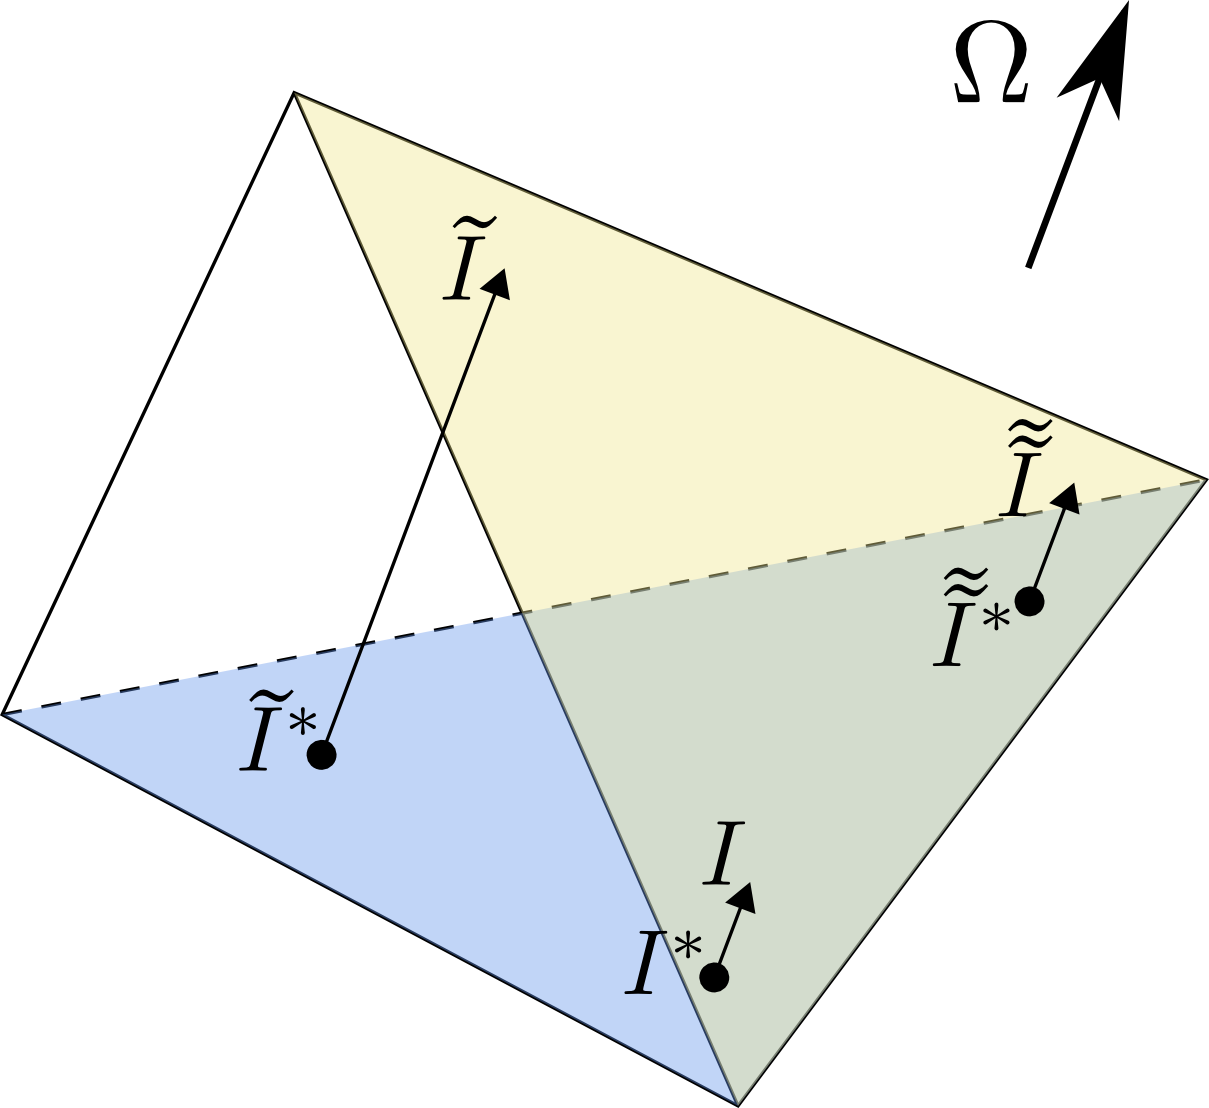
\includegraphics[width = 0.5\textwidth]{slide72.png}
}
\caption{К построению метода коротких характеристик}
\label{fig:3}
\end{figure}

Каждое из уравнений \eqref{8} является гиперболическим и для его решения можно применить сеточно-характеристический метод. Для вычисления интенсивности $I_{\nu,i}$ в точке $p$ выпускается луч в направлении $-\vec\omega_i$ до пересечения с первой гранью. В точке пересечения $\vec r^*$ вычисляется интерполированное по вершинам грани значение интенсивности $I_{\nu, i} (\vec r^*) = \sum_{j = q,r,s} \alpha_jI_{\nu, i}(\vec r_j)$. Далее, $I_{\nu, i} (\vec r_p)$ вычисляется из решения одномерного уравнения переноса   
\begin {equation}
I_{\nu}(s) = \int_{s_0}^s\varkappa'_{\nu}I_{\nu p} \exp\Big[-\int_{s'}^s\varkappa'_{\nu}ds''\Big]ds' + I_{\nu,0} \exp\Big[-\int_{s_0}^s \varkappa'_{\nu}ds''\Big].
\end {equation}

В простом случае, если в тетраэдре $\varkappa_\nu = \operatorname{const}$, формула упрощается до 
\begin {equation}
I_\nu (s) = I_{\nu p} \left(1 - e^{-\varkappa_\nu \Delta}\right) + I_{\nu,0}e^{-\varkappa_\nu \Delta},
\end {equation}
где $\Delta = s - s_0$. Очевидно, что $I_\nu(s)$ лежит в пределах от $I_{\nu, 0}$ до $I_{\nu p}$
\section {Многогрупповое приближение}
Разобъем весь спектр на конечное число $N_k$ интервалов по частоте - групп. Внутри каждой группы для частот $\nu$, лежащих в пределах $\nu_k \leqslant \nu \leqslant \nu_{k+1}$, $\nu_1 = 0$, $\nu_{N_k} = \infty$, будем предполагать, что коэффициент поглощения не зависит от энергии фотона:
\begin {equation}
\varkappa_\nu (T, \rho, \nu) = \varkappa_k(t, \rho), \quad \nu_k \leqslant \nu \leqslant \nu_{k+1}, \quad k = 1 \div N_k.
\label{10}
\end {equation}
Интегральный потом и плотность энергии излучения представим в виде
\begin {equation}
\vec W = \int_0^\infty d\nu \int \vec\Omega I_\nu d\Omega = \sum_{k=1}^{N_k} \int \vec\Omega I_k d\Omega, \quad I_k = \int_{\nu_k}^{\nu_{k+1}} I_\nu d \nu, 
\end {equation}
\begin {equation}
U = \frac{1}{c} \int_0^\infty d\nu \int I_\nu d \Omega = \sum_{k=1}^{N_k} \frac{1}{c} \int I_k d \Omega.
\end {equation}
Для определения уравнения, которому удовлетворяет $I_k$, проинтегрируем уравнение переноса по $\nu$ от $\nu_k$ до $\nu_{k+1}$. Учитывая, что коэффициент поглощения \eqref{10} в этом диапазоне не зависит от частоты, получим
\begin {equation}
(\vec\Omega \nabla )I_k + \varkappa_k I_k = \varkappa_k \int_{\nu_k}^{\nu_{k+1}} I_{\nu, p} d \nu.
\end {equation}
Многогрупповое приближение позволяет рассматривать уравнение переноса как уравнение относительно вектор-функции $\vec I $ интенсивности излучения, компоненты которой являются значением интенсивности в своей частотной группе. 
После преобразования уравнения \eqref{2} получим
\begin {equation}
(\vec\Omega \nabla ) \vec I + \vec K \vec I = \vec K \vec I_{p},
\end {equation} 
где $\vec K = diag \varkappa_k$. Если рассматривать это уравнение как векторное, то можно избежать повторения одинаковых геометрических вычислений для каждой частоты.
\section{Маршевый метод}
Разделим грани тетраэдра на входящие и выходящие \ref{fig:4}. Грань называется входящей, если луч, пересекающий ее, входит в тетраэдр, в противном случае~--- выходящей. Решение на выходящих гранях тетраэдра можно найти только тогда, когда решение на входящих гранях уже посчитано. Соответственно, на гранях триангуляции образуется отношение частичного порядка. В случае, если это отношение не образует цикл, его можно распространить на все множество граней, то есть задать такой порядок обхода граней, при котором выходные грани каждого тетраэдра идут после входных граней этого же тетраэдра. 

\begin{figure}[ht!]
\centering{
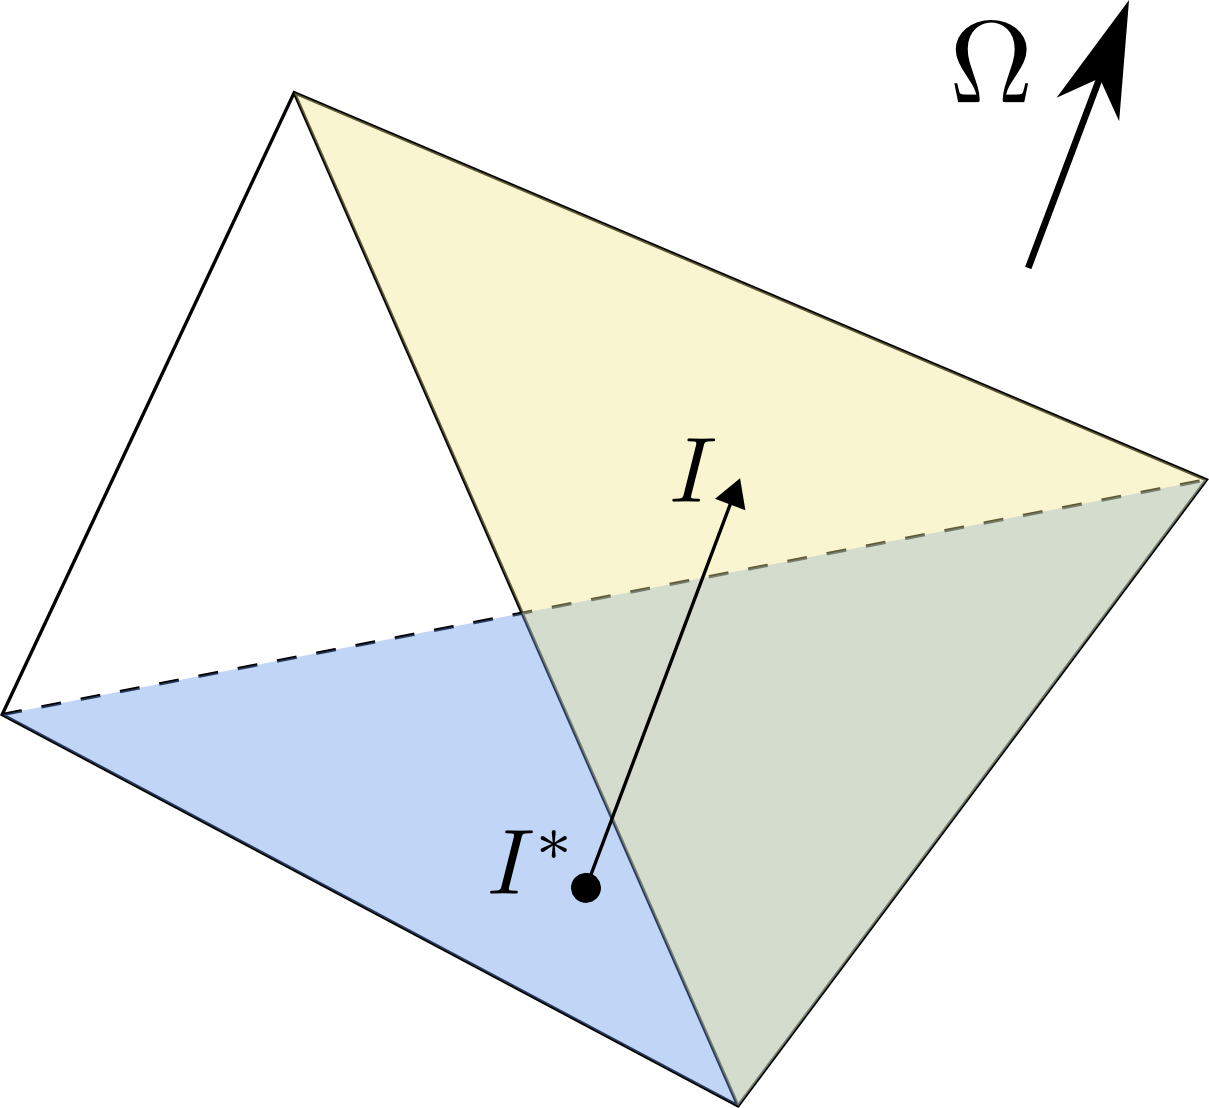
\includegraphics[width = 0.7\textwidth]{slide71.png}
}
\caption{Входящие и выходящие грани тетраэдра.}
\label{fig:4}
\end{figure}

Для триангуляции Делоне порядок, в котором свет проходит грани такой же, в котором свет проходит центры описанных вокруг тетраэдра сфер, и требуемый порядок можно получить сортировкой координат центров тетраэдров вдоль направления переноса излучения \cite{skalko_2014}.

В случае, если триангуляция не является триангуляцией Делоне, такая сортировка может привести к неверному результату: могут образоваться тетраэдры, в которых выходные грани проходятся раньше входных. Однако задача упорядочения граней решается для более широкого класса, чем класс триангуляций Делоне. 

Предлагается следующий алгоритм упорядочения, являющийся адаптацией поиска в ширину. Частичный порядок граней порождает отношение порядка тетраэдров. Нужно пометить тетраэдры номером так, чтобы отношение порядка было связано соответственно с возрастанием номера тетраэдра. Пусть $c(T)$ - номер (цвет) тетраэдра $T$. Тогда условие упорядоченности можно записать как $ c(T) > c (T')$ для всех $T'$, граничащих с $T$ по входной грани. 

Есть очередь тетраэдров, из которой извлекаются и в которую добавляются тетраэдры. В очереди сначала находятся все тетраэдры, грани которых были освещены. За шаг алгоритма из очереди извлекается один тетраэдр, проверяется, все ли его входящие грани освещены. В этом случае тетраэдр удаляется из очереди, а в очередь добавляются все его неосвещенные соседи. Если это не так, тетраэдр добавляется в конец очереди. При работе с очередью производится проверка на цикл: если обнаруживается, что из очереди нельзя удалить ни один тетраэдр, значит, в триангуляции имеется цикл, и алгоритм останавливается (дальнейшее использование маршевого метода невозможно).

Кроме самого упорядочения этот алгоритм группирует грани, решения на которых могут быть вычислены параллельно в силу своей независимости друг от друга. Это может стать основой для последующего распараллеливания алгоритма.
\section{Особенности выбора точек на грани}
Точки, из которых выпускаются характеристики на грани, не могут быть взяты произвольно. Рассмотрим данный метод, примененный к одномерному не стационарному уравнению переноса.

\begin {equation}
\frac{\partial u}{\partial t} + \frac{\partial u}{\partial x} = 0
\end {equation}

На каждом ребре решение является линейной функцией $u_i^n(x) = \alpha_i^nx+\beta_i^n $. Со слоя $n+1$ на $n$ выпускаются две характеристики, на которых решение сохраняется. На слое $n+1$ решается система относительно $\alpha_i^{n+1}$ и $\beta_i^{n+1}$. 

\begin{figure}[ht!]
\centering{
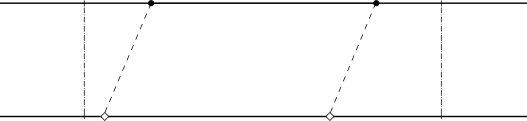
\includegraphics[width = 0.5\textwidth]{bad_char.png}
}
\caption{Положение характеристик при $\sigma < \sigma_\text{кр}$}
\label{fig:5}
\end{figure}
Числом Куранта для этой задачи будет $\tau/h$, а $\sigma_\text{кр} = h_1/h$. Когда число Куранта $\sigma < \sigma_\text{кр}$, схема теряет устойчивость, так как решение не может покинуть ячейку (см. рис. \ref{fig:5}). Такого эффекта нет, если характеристики выпускаются из узлов расчетной сетки. Он проявляется на прямоугольных сетках, неизвестно, какой эффект он окажет на неструктурированные. В связи с этим в используемом методе в набор точек, из которых испускается характеристики, всегда включаются вершины граней. 
\section{Повышение порядка пространственной аппроксимации. Монотонная интерполяция}
В случае использования минимального количества (трех вершин на каждой грани), получается метод первого порядка, который имеет существенную численную диффузию луча. Получается схема первого порядка, чтобы увеличить точность схемы, используются дополнительные точки на гранях. В качестве таких точек выбираются середины ребер. 

Использование интерполяции на гранях по шести точкам позволяет поднять порядок аппроксимации метода коротких характеристик до второго. Такая параболическая интерполяция имеет существенный недостаток: она не является монотонной, то есть потенциально может приводить к появлению отрицательных значений интенсивности, что лишено физического смысла  \ref{8}. Для того, чтобы избежать немонотонной интерполяции, нужно использовать процедуру ограничения решения в серединах ребер, исходя из соображения, что экстремум параболы должен находиться либо в вершинах ребра, либо за его пределами. 
\begin{figure}[ht!]
	\centering{
		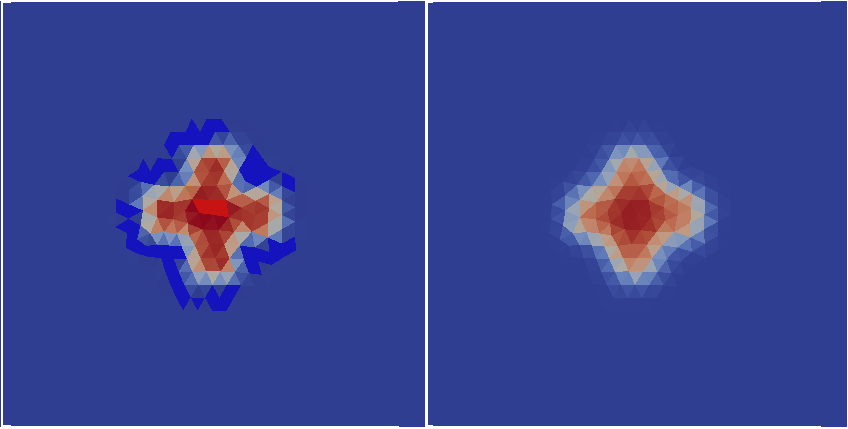
\includegraphics[width = 0.5\textwidth]{2vs2lim.png}
	}
	\caption{Сравнение методов второго порядка и второго с ограничителем}
	\label{fig:8}
\end{figure}
Для этого рассмотрим отрезок $[-1, 1]$. Предполагается, что значение в концах отрезка известны и равны соотвественно $I_1$ и $I_2$. Решение в центре обозначим как $I_{mid}$. Из условия на экстремум следует, что абсцисса вершины параболы должна удовлетворять условию $|x_{\text{верш}}| \geqslant 1 $. Учитывая, что парабола в общем виде $ax^2 + bx + c = 0$ и с нашими условиями имеет следующие коэффициенты:
\begin {equation}
a = \frac{I_1 + I_2 - 2I_{mid}}{2}, \quad b = \frac{I_2 - I_1}{2}, \quad c = I_{mid}, 
\end {equation}
а $x_{\text{верш}} = -\frac{b}{2a}$, получим, что
\begin {equation}
\left| \frac{I_1 - I_2}{2(I_1 + I_2 - 2I_{mid})}\right| \geqslant 1,
\end {equation}
откуда элементарными преобразованиями получаем условие на центр ребра:
\begin {equation}
\left| I_{mid} - \frac{I_1 + I_2}{2}\right| \leqslant \left| \frac{I_1 - I_2}{4}\right| .
\end {equation}
При $a=0$ парабола становится прямой, у нее нет экстремума, следовательно, полученное условие будет верно. 
В численном методе значение интенсивности на ребрах ограничиваются по ближайшей границе допустимого интервала. Для выявления разницы между схемами первого и второго порядка аппроксимации использовались также кусочно-линейная интерполяция интенсивности по шести точкам. Это позволяет сравнить метод первого и второго порядка при одинаковом количестве (степеней свободы) узловых точек. 

В качестве базиса для квадратичной интерполяции используются функции $\ell_0 \div \ell_5$, которые в стандартном треугольнике  имеют вид:

\begin {equation}
\begin {aligned}
\ell_0 (\xi, \eta)&= (\eta + \xi -1)(2\eta + 2\xi - 1) \\
\ell_1 (\xi, \eta)&= \xi(2\xi - 1) \\
\ell_2 (\xi, \eta)&= \eta (2\eta - 1) \\
\ell_3 (\xi, \eta)&= 4\eta\xi \\
\ell_4 (\xi, \eta)&= -4\eta(\eta + \xi - 1) \\
\ell_5 (\xi, \eta)&= -4\xi(\eta + \xi - 1) \\
\end {aligned}
\end {equation}

Для интерполяции первого порядка для тех же шести точек используются следующие базисные функции:

\begin {equation}
\begin {aligned}
\ell_0 (\xi, \eta) &= 
\begin{cases}
0, & \xi + \eta \geqslant 0.5 \\
1-2(\xi + \eta), & \xi + \eta < 0.5
\end{cases}
 \\
\ell_1 (\xi, \eta) = \ell_2 (\eta, \xi) &= 
\begin{cases}
0, & \xi < 0.5 \\
2\xi - 1, & \xi > 0.5
\end{cases}
\\
\ell_3 (\xi, \eta) &=
\begin{cases}
0, & \xi + \eta < 0.5 \\
2\eta, & \xi > 0.5 \\
2\xi, &\eta > 0,5 \\
2\xi + 2\eta - 1, & \text{иначе}
\end{cases}
\\
\ell_4 (\xi, \eta) = \ell_5(\eta, \xi)&= 
\begin{cases}
2\eta, & \xi + \eta < 0.5 \\
0, & \xi > 0.5 \\
-2\xi -2\eta + 2, &\eta > 0,5 \\
-2\xi + 1, & \text{иначе}
\end{cases}
\\
\end {aligned}
\end {equation}

Причем, для случая первого порядка коррекция значений на ребрах не требуется.
% Глава 3
\chapter{Результаты}

\section{Сравнение методов первого и второго порядка}
\subsection{Решение уравнения в одном направлении}
Сравнение методов проводилось на следующей задаче. Рассматривалась
геометрическая область, куб со стороной $a = 2$. В центре области находится
крест, состоящий из пяти одинаковых кубиков со стороной $b = 0.2$ (см. рис. \ref{fig:6}).
\begin{figure}[ht!]
\centering{
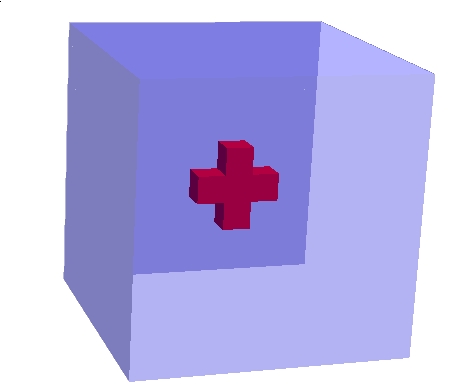
\includegraphics[width = 0.5\textwidth]{cross.png}
}
\caption{Расчетная область.}
\label{fig:6}
\end{figure}
Коэффи\-циент поглощения в области равен $\varkappa_1=0$, а внутри креста --- $\varkappa_2 = 100$. Равновесная интенсивность в центральной области $1$, а в окружающей среде --- $0$. Решение строилось вдоль одного направления, $\omega = (0,0,1)$ на сетке с $415625$ тетраэдрами и $76247$ вершинами. Изучалось решение на выходной грани куба. 
\begin{figure}[ht!]
\centering{
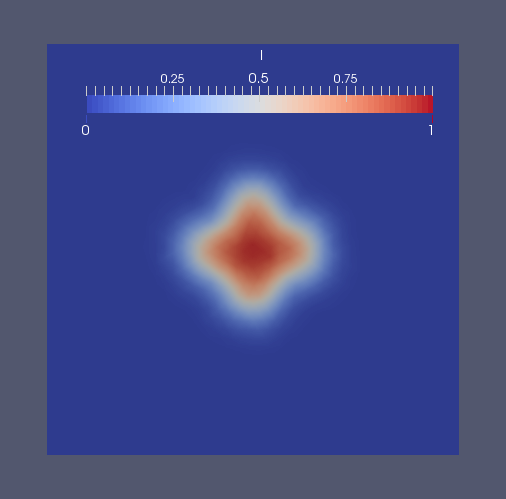
\includegraphics[width = 0.3\textwidth]{1ord.png}%
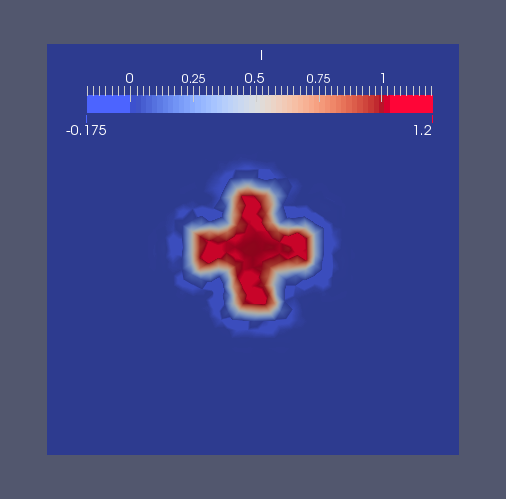
\includegraphics[width = 0.3\textwidth]{2nolim.png}%
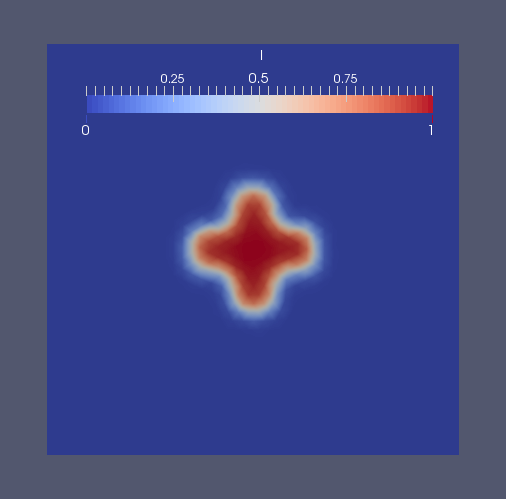
\includegraphics[width = 0.3\textwidth]{2wilim.png}
}
\caption{Сравнение решений методами первого порядка (слева), второго (в центре) и второго с ограничителем(справа).}
\label{fig:7}
\end{figure}

Точное решение должно представлять собой крест с интенсивностью $1 -
e^{b\varkappa_2} = 1-e^{-20} \approx 1$. Мы можем видеть (см. рис. \ref{fig:7}), что для первого порядка диффузия достаточно велика, второй порядок без ограничителя отклоняется от допустимых пределов $I \in [0, 1]$ на $20 \%$.
\subsection{Сравнение плотности излучения}
На той же самой задаче изучалась плотность излучения в центральном сечении куба, но коэффициенты поглощения изменились следующим образом: $\varkappa_1 = 10$, $\varkappa_2 = 1$. . Использовались 170 направлений из квадратурной формулы Лебедева \cite{lebedev_1999}. 

\begin{figure}[ht!]
\centering{
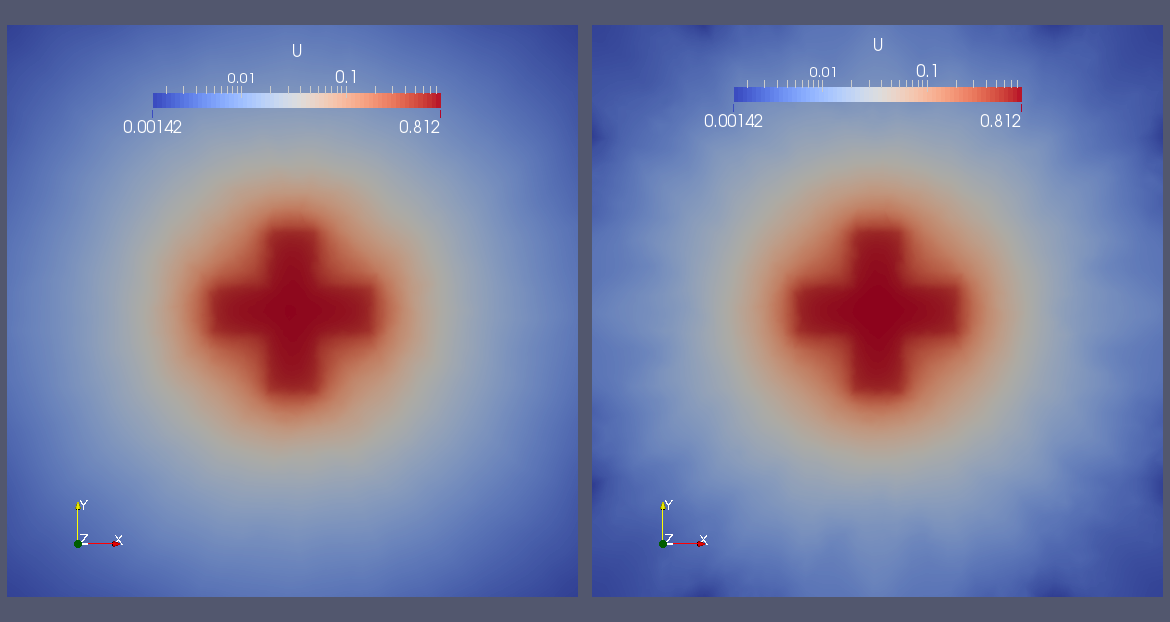
\includegraphics[width = \textwidth]{U2vs1.png}
}
\caption{Сравнение плотности излучения в центральном сечении куба. Слева второй порядок, справа --- первый.}
\label{fig:9}
\end{figure}

\begin{figure}[ht!]
\centering{
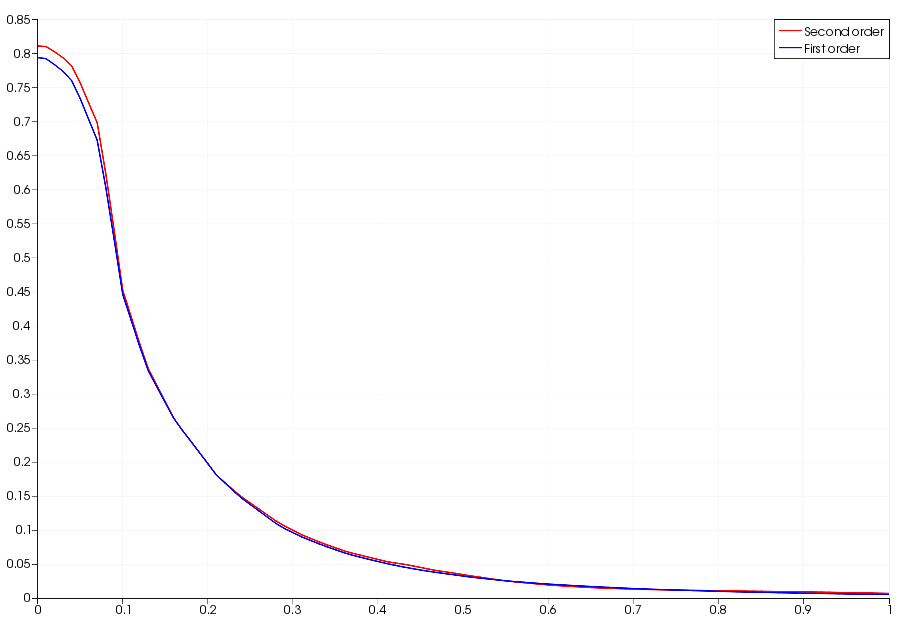
\includegraphics[width = \textwidth]{U2vs1Line.png}
}
\caption{Плотность излучения вдоль оси $Oz$. Красный второй порядок, синий - первый.}
\label{fig:10}
\end{figure}
Сравнение плотности излучения \ref{fig:9} и \ref{fig:10} показывает схожие результаты: интенсивность в центре куба в методе второго порядка на $\approx 2 \%$ больше, чем в случае метода первого порядка. В случае метода второго порядка \ref{fig:9} более выражен <<эффект луча>>, в то время как в методе первого порядка этот эффект сглажен за счет численной диффузии. 

\section{Сравнение методов первого и второго порядка с одинаковым количеством степеней свобод}
Рассматривалась геометрическая область: две концентрические сферы  с центром в точке $(0,0,0)$, внешняя радиусом $R = 5$, а внутренняя --- $r = 0.35$ (см. рис. \ref{fig:11}). Коэффициент поглощения между  сферами равен $\varkappa_1 = 0$, а внутри меньшей сферы --- $\varkappa_2 = 10$. Равновесная интенсивность в центральной области $1$, а в окружающей среде --- $0$. 
\begin{figure}[ht!]
\centering{
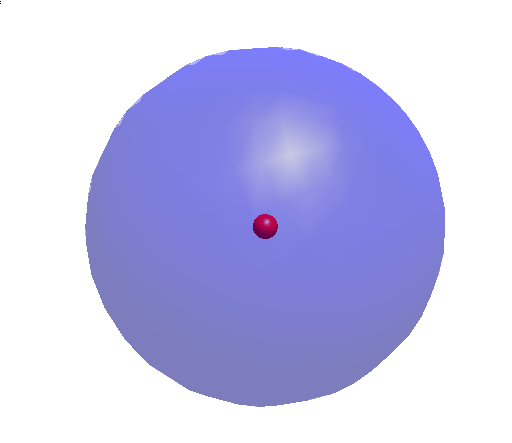
\includegraphics[width = 0.5\textwidth]{sphere.png}
}
\caption{Расчетная область в случае сравнения методов первого и второго порядка с одинаковым количеством степеней свобод.}
\label{fig:11}
\end{figure}
Решение строилось вдоль одного направления $\omega = (1, 0, 0)$ на сетке с $387736$ тетраэдрами и $70705$ точками. Изучалось решение в центральном сечении. 
\begin{figure}[ht!]
\centering{
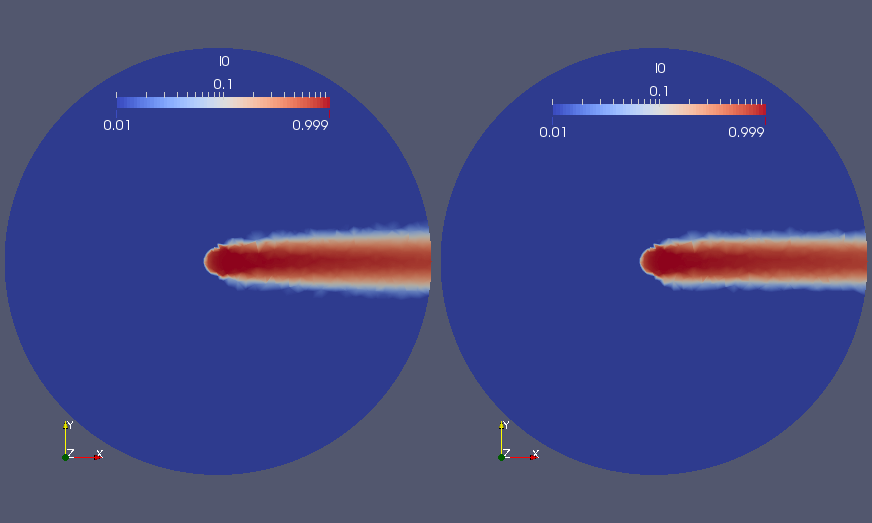
\includegraphics[width = 0.7\textwidth]{2vs15.png}
}
\caption{Диффузия луча в методе первого (справа) и второго (слева) порядка при одинаковом количестве степеней свободы.}
\label{fig:12}
\end{figure}

Увеличение количества степеней свободы делает метод первого порядка практически таким же точным, как и метод второго порядка, однако численное рассеяние луча имеет различный характер в обоих случаях (см. рис. \ref{fig:12}). В случае метода второго порядка оно практически не меняется вдоль луча, в то время как для метода первого порядка оно растет пропорционально корню удаления от источника ($\Delta y^2 \sim x$), как и должно быть в случае метода первого порядка. 
\section{Моделирование спектра излучения звезды при наличии конического ветра}
Уравнение переноса решалось по результатом МГД моделирования взаимодействия звезды типа Т-Тельца с ее аккреционным диском, проведенного в работе \cite{rom_2009}. В численном МГД моделировании наблюдался сильный так называемый конический ветер (см. рис. \ref{fig:15} справа). 
\begin{figure}[ht!]
\centering{
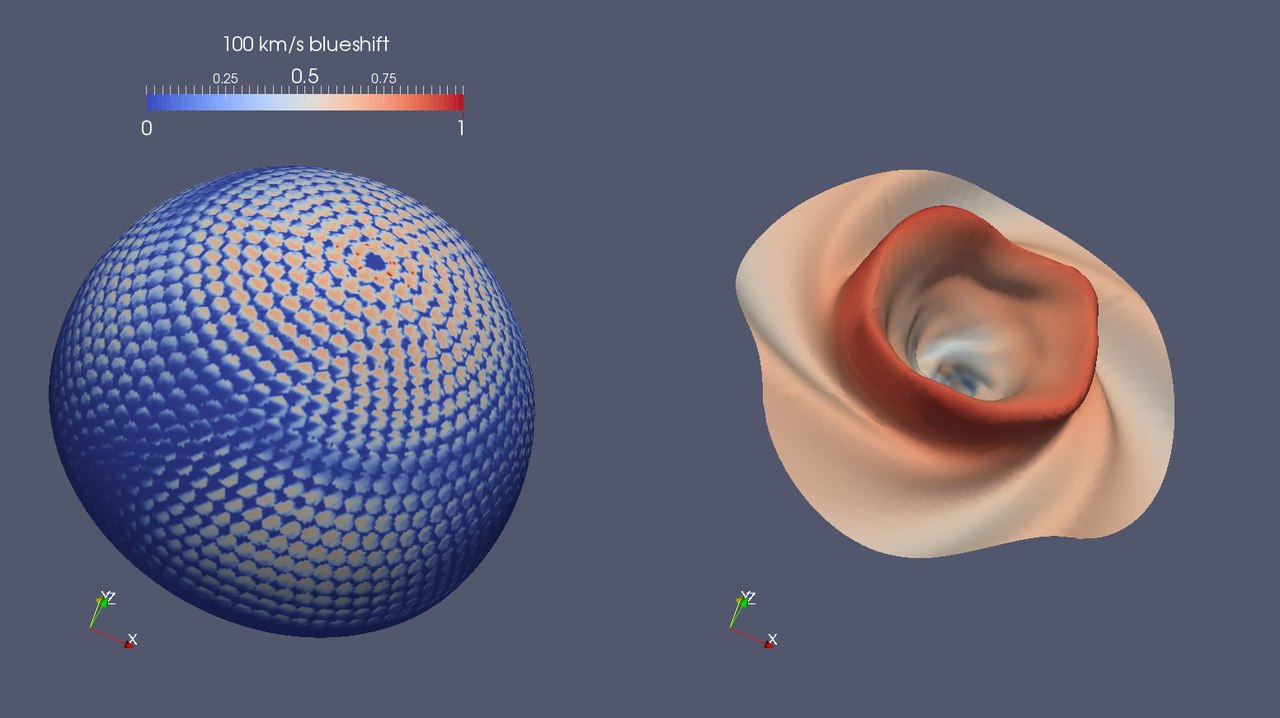
\includegraphics[width = 0.7\textwidth]{star.jpg}
}
\caption{Слева интенсивности излучения звезды в различных направлениях на частоте, соответствующей синему смещению в $180 \text{ км/с}$. Справа - изоповерхность плотности вещества.}
\label{fig:15}
\end{figure}

Уравнение переноса решалось с использованием $1091$ направления и $64$ частотных групп, соответствующих доплеровскому смещению от $-600 \text{ км/с}$ до $600 \text{ км/с}$. Источником излучения служит сама звезда, находящаяся в центре области. Спектр излучения звезды соответствует линии водорода $\text{H}\alpha$, испытывающей тепловое доплеровское уширение с температурой $T = 4.6 \cdot 10^6 \text{ K}$. Равновесное излучение в окружающем звезду пространстве считается отсутствующем. Коэффициенты поглощения рассчитывались в приближении локального термодинамического равновесия. 

 На рисунке \ref{fig:15} слева изображено объединение интенсивностей воль каждого из исследуемых направлений. На частоте, соответствующей синему смещению в $180 \text{ км/с}$, наблюдается значительное поглощение в тех направлениях, которые проходят через область конического ветра. На рисунке \ref{fig:16} значительное поглощение можно наблюдать для спектральных групп, соответствующих скоростям $\Delta v = -194 \text{ км/с}$ и $\Delta v = -157 \text{ км/с}$ при угле наклонения $45^\circ$.
 
 \begin{figure}[ht!]
 \centering{
 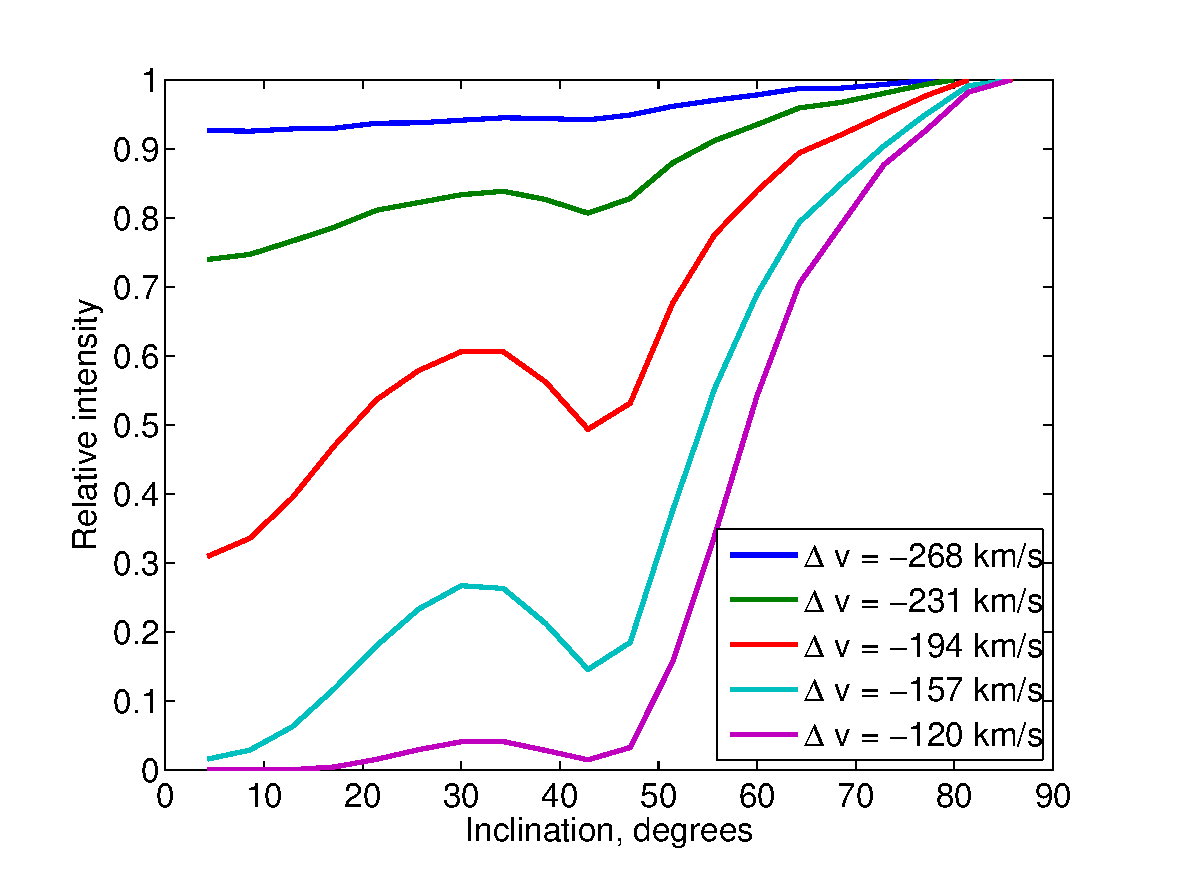
\includegraphics[width = 0.7\textwidth]{varinc.eps}
 }
 \caption{Средняя за период обращения относительная интенсивность излучения на разных частотах в зависимости от угла наклонения Земли по отношению к плоскости вращения звезды.}
 \label{fig:16}
 \end{figure} 

% Заключение
\conclusion
Построен маршевый вычислительный алгоритм для решения стационарной задачи переноса излучения на неструктурированной трехмерной сетке во многогрупповом приближении. В основе маршевого метода лежит алгоритм упорядочения тетраэдров. В данной работе построен более универсальный алгоритм упорядочения тетраэдров, чем описанный в \cite{skalko_2014}, так как работает для более широкого класса триангуляций, чем триангуляции, удовлетворяющие условию Делоне.

Было найдено необходимое условие устойчивости данного численного метода, применительно к модельной задаче на равномерной сетке. Был реализован метод второго порядка аппроксимации и его монотонная модификация. 

Проведено сравнение методов на различных модельных задачах. Показано, что немонотонный вариант метода второго порядка может иметь нефизические осцилляции величиной порядка $20 \%$. Продемонстрировано различное качественное поведение численной диффузии излучения для методов первого и второго порядков аппроксимации.

Вычислительный алгоритм был применен к прикладной задаче воспроизведения спектра излучения звезды по результатам МГД моделирования взаимодействия магнитного поля звезды с веществом аккреционного диска. 

% Список литературы
\bibliography{thesis}
\bibliographystyle{utf8gost71u}

% Приложения
\appendix
\chapter{Заголовок приложения}


\end{document}
